\documentclass[tikz]{standalone}
\usepackage{amsmath}
\usepackage{pgfplots}
\usepackage{times}
\usepackage{txfonts}

\usetikzlibrary{arrows,intersections,math}

\begin{document}
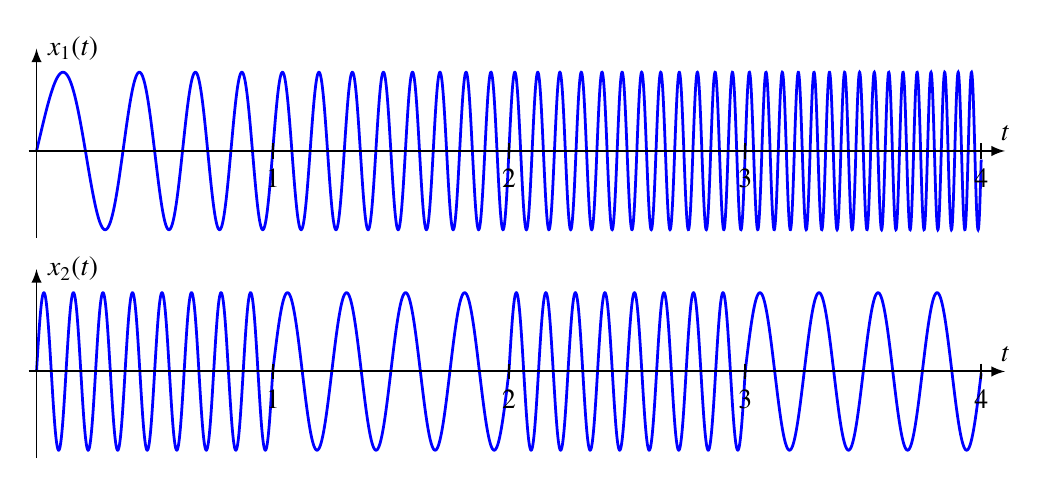
\begin{tikzpicture}[>=latex]

	\pgfmathparse{12/4} % scale to tend
	\xdef\a{\pgfmathresult} 
	
	\begin{scope}[yshift=1.4cm]
		\draw[color=blue,line width=1pt]
		plot[domain=0:4,samples=4000, smooth]
		({\x*\a},{sin(360*\x*(2 + 6/\a * \x))});
		\draw[->,line width=0.7pt] (-0.1,0)--(12.3,0) coordinate[label={$t$}];
		\draw[->,line width=0.7pt] (0,-1.1)--(0,1.3) coordinate[label={right:$x_1(t)$}];
		
		\foreach \x in {1,...,4}{
			\draw[line width=0.7pt] ({\x*\a},0.1) --({\x*\a},-0.1) coordinate[label={below:$\x$}];
		}
	\end{scope}
	
	\begin{scope}[yshift=-1.4cm]
		\draw[color=blue,line width=1pt]
		plot[domain=0:4,samples=4000, smooth]
		({\x*\a},{sin(360*\x*(6 + 2 * sign(sin(180*\x)) ))});
		\draw[->,line width=0.7pt] (-0.1,0)--(12.3,0) coordinate[label={$t$}];
		\draw[->,line width=0.7pt] (0,-1.1)--(0,1.3) coordinate[label={right:$x_2(t)$}];
		
		\foreach \x in {1,...,4}{
			\draw[line width=0.7pt]	({\x*\a},0.1)--({\x*\a},-0.1) coordinate[label={below:$\x$}];
		}
	\end{scope}

\end{tikzpicture}

\end{document}
